\section{Entropia Contínua/Diferencial}

\begin{frame}[allowframebreaks]
  \frametitle{Entropia}
  \begin{itemize}
  \item Caso discreto
	\begin{equation}
	H(X) = - \sum_x p(x) \log p(x)
	\end{equation}
  \item O mundo é contínuo, os canais são contínuos, ruído é contínuo.
  \item Precisamos de uma teoria que possa ser aplicada ao domínio contínuo.
  \end{itemize}
\end{frame}


\begin{frame}[allowframebreaks]
  \frametitle{Entropia Contínua/Diferencial}
  \begin{itemize}
  \item Seja $X$ uma v.a. contínua com distribuição cumulativa
	\begin{equation}
	F(x) = \Pr (X \leq x)
	\end{equation}
	e a função densidade é dada pela derivada da cumulativa
	\begin{equation}
	f(x) = \frac{d}{dx} F(x) .
	\end{equation}
  \item O suporte é definido por $S = \{ x: f(x) > 0 \}$.
	\begin{definition}[entropia diferencial $h(X)$]
	\begin{equation}
	h(X) = - \int_S f(x) \log f(x) dx
	\end{equation}
	\end{definition}
  \item Como a integral é sobre o suporte $S$, não precisamos nos preocupar com $\log 0$.
  \end{itemize}

  \framebreak

  \begin{example}
  Dado $X \sim \mathcal{U}[0,a]$ com $a \in R^+$, teremos
	\begin{equation}
	h(X) = - \int_{0}^{a} \frac{1}{a} \log \frac{1}{a} dx = - \log \frac{1}{a} = \log a
	\end{equation}
  \begin{itemize}
  \item Dependendo do valor de $a$, podemos ter entropia com valor positivo ou negativo, e ainda não é limitada.
  \end{itemize}
  \end{example}
  \begin{itemize}
  \item Entropia pode ser interpretada como o expoente do `volume' do conjunto típico. Por exemplo,
	$2^{nH(X)}$ é o número de eventos que ocorrem, em média; podemos ter $2^{H(X)} \ll \vert \mathcal{X} \vert$.
	Teremos igualdade no caso uniforme. A incerteza de uma v.a. $X$ é equivalente à de uma
	v.a. uniforme $Y$ tal que $2^{H(X)} = \vert \mathcal{Y} \vert$.
  \item Expoente negativo significa que o `volume' é pequeno.
  \end{itemize}

  \framebreak

  \begin{example}
  Distribuição Normal (Gaussiana).
  Seja a v.a. $X \sim \mathcal{N}(0, \sigma^2)$, densidade dada por 
	\begin{equation}
	f(x) = \frac{1}{(2\pi \sigma^2)^{1/2}} e^{-\frac{1}{2} x^2 / \sigma^2}
	\end{equation}
  \begin{itemize}
  \item Intuitivamente, sabemos que a entropia não depende da média $\mu$.
  \end{itemize}
  \examplebreak
  \begin{itemize}
  \item Calculando a entropia em nats
	\begin{eqnarray}
	h(X) &=& - \int f(x) \ln f(x) dx \\ 
		&=& - \int f(x) \left[ - \frac{x^2}{2\sigma^2} - \ln \sqrt{2\pi \sigma^2}\right] dx \\
		&=& \frac{\E X^2}{2\sigma^2} + \frac{1}{2} \ln (2 \pi \sigma^2) = \frac{1}{2} + \frac{1}{2} \ln (2 \pi \sigma^2) \\
		&=& \frac{1}{2} \ln e + \frac{1}{2} \ln (2 \pi \sigma^2) = \frac{1}{2} \ln (2 \pi e \sigma^2) \text{nats} \\
		&=& \frac{1}{2} \ln (2 \pi e \sigma^2) \text{nats} \times \left( \frac{1}{\ln 2} \text{bits/nats} \right) = \frac{1}{2} \log (2 \pi e \sigma^2) \text{bits}. \nonumber
	\end{eqnarray}
  \end{itemize}
  \end{example}
\end{frame}

\subsection{Propriedade da Equipartição Assintótica}
\begin{frame}[allowframebreaks]
  \frametitle{Propriedade da Equipartição Assintótica}
  \begin{itemize}
  \item  No caso discreto: $\Pr(x_1, x_2, \ldots, x_n) \approx 2^{-nH(X)}$ para $n$ grande suficiente
	e $\vert A_{\epsilon}^{(n)} \vert = 2^{nH} = (2^H)^n$.
  \item Desta forma, $2^H$ pode ser visto como o `comprimento do lado' de um hipercubo em um espaço $n$ dimensional,
	e assim $2^{nH}$ seria o volume deste hipercubo (ou volume do conjunto típico).
  \item $H$ negativo implicaria em um comprimento pequeno $2^H$, mas ainda positivo.
  \end{itemize}

  \framebreak

  \begin{theorem}
  Seja $X_1, X_2, \ldots, X_n$ uma sequência de v.a.s, i.i.d. $\sim f(x)$, então
	\begin{equation}
	- \frac{1}{n} \log f(X_1, \ldots, X_n) \rightarrow \E \left[ - \log f(X) \right] = h(X)
	\end{equation}
  \end{theorem}

  \begin{definition}[Conjunto Típico]
	\begin{equation}
	A_{\epsilon}^{(n)} = \left\{ x_{1:n} \in S^n : \vert -\frac{1}{n} \log f(x_1, \ldots, x_n) - h(X) \vert \leq \epsilon \right\}
	\end{equation}
  \end{definition}
  \begin{itemize}
  \item Note que 
	\begin{equation}
	f(x_1, \ldots, x_n) = \prod_{i=1}^n f(x_i) .
	\end{equation}
  \item Limites para esta probabilidade
	\begin{equation}
	2^{-n(h + \epsilon)} \leq f(x_{1:n}) \leq 2^{-n(h - \epsilon)}
	\end{equation}
  \item O volume de $A \subseteq \RealNumber^n$ é definido
	\begin{equation}
	\text{Vol}(A) = \int_A dx_1 dx_2 \ldots dx_n
	\end{equation}
  \end{itemize}

  \begin{theorem}
  \begin{enumerate}
  \item Probabilidade do conjunto típico
	\begin{equation}
	\Pr( A_{\epsilon}^{(n)} ) > 1 - \epsilon
	\end{equation}
  \item Volume do conjunto típico
	\begin{equation}
	(1-\epsilon) 2^{n(h(X) - \epsilon)} \leq \text{Vol}(A_{\epsilon}^{(n)}) \leq 2^{n(h(X)+\epsilon)}
	\end{equation}
  \end{enumerate}
  \end{theorem}
  \begin{itemize}
  \item Temos limites no volume do conjunto típico.
  \item No caso discreto, os limites eram sobre a cardinalidade do conjunto típico, e neste caso
	era necessário $H(X) \geq 0$, pois o tamanho mínimo de $\vert A_{\epsilon}^{(n)} \vert$ é 1.
  \end{itemize}

  \framebreak

  \begin{proof}
  Por definição
  \begin{eqnarray}
	p(A_{\epsilon}^{(n)}) &=& \int_{x_{1:n} \in A_{\epsilon}^{(n)}} f(x_1, \ldots, x_n) dx_1 \ldots dx_n \\
		&=& \Pr \left( \vert - \frac{1}{n} f(x_1,x_2,\ldots,x_n) - h(X) \vert \leq \epsilon \right) \geq 1 - \epsilon \nonumber
  \end{eqnarray}
  	para $n$ grande suficiente, o que segue da lei fraca dos grandes números.

  \proofbreak
  Temos também que
  \begin{eqnarray}
	1 &=& \int_{S^n} f(x_1, \ldots, x_n) dx_1 \ldots dx_n \geq \int_{A_{\epsilon}^{(n)}} f(x_1, \ldots, x_n) dx_1 \ldots dx_n \nonumber \\
		&\geq& \int_{A_{\epsilon}^{(n)}} 2^{-n(h(X) + \epsilon)} dx_{1:n} = 2^{-n(h(X) + \epsilon)} \text{Vol}(A_{\epsilon}^{(n)})
  \end{eqnarray}
  Logo,
	\begin{equation}
	 \text{Vol}(A_{\epsilon}^{(n)}) \leq 2^{n(h(X) + \epsilon)}
	\end{equation}

  \proofbreak 
  De forma similar,

  \begin{eqnarray}
  1 - \epsilon &\leq& \Pr(A_{\epsilon}^{(n)}) = \int_{A_{\epsilon}^{(n)}} f(x_{1:n}) dx_{1:n} \\
	&\leq& \int_{A_{\epsilon}^{(n)}}  2^{-n(h(X) - \epsilon)} dx_{1:n} =  2^{-n(h(X) - \epsilon)} \text{Vol}(A_{\epsilon}^{(n)})
  \end{eqnarray}
  \end{proof}

  \begin{itemize}
  \item $A_{\epsilon}^{(n)}$ é o menor volume que contém toda a probabilidade e este volume é $\approx 2^{nh}$, e 
	o tamanho do lado deste hipercubo é $2^h$.
  \item Portanto, faz sentido $- \infty < h < \infty$.
  \end{itemize}
\end{frame}

\subsection{Entropia Discreta vs Diferencial}
\begin{frame}[allowframebreaks]
  \frametitle{Entropia Discreta vs Entropia Diferencial}
  \begin{itemize}
  \item Seja $X \sim f(x)$. Vamos dividir a extensão de $X$ em \textit{bins} (caixas) de tamanho $\Delta$.
  \item Quantizar a extensão de $X$ utilizando $n$ bits, assim $\Delta = 2^{-n}$.
                \begin{figure}[h!]
                \centering
                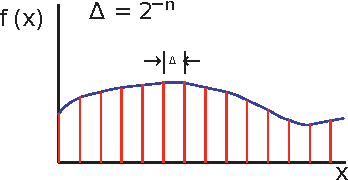
\includegraphics[width=0.5\textwidth]{images/xbins.pdf}
                \label{fig:xbins}
                \end{figure}
  \item Pelo teorema do valor médio, se $f(\cdot)$ é contínua em um intervalo $[i\Delta, (i+1)\Delta]$, então $\exists x_i$
	dentro deste intervalo, tal que
	\begin{equation}
	f(x_i) = \frac{1}{\Delta} \int_{i\Delta}^{(i+1)\Delta} f(x) dx
	\end{equation}
                \begin{figure}[h!]
                \centering
                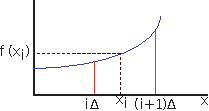
\includegraphics[width=0.5\textwidth]{images/teovalmed.pdf}
                \label{fig:teovalmed}
                \end{figure}
  \item Vamos criar uma variável aleatória quantizada $X^\Delta$ com os seguintes valores
	\begin{equation}
	X^\Delta = x_i \quad \text{ se } i \Delta \leq X \leq (i+1) \Delta
	\end{equation}
  \item Obtemos assim a distribuição discreta
	\begin{equation}
	\Pr (X^\Delta = x_i) = p_i = \int_{i\Delta}^{(i+1)\Delta} f(x) dx = \Delta f(x_i)
	\end{equation}
	podemos calcular a entropia
	\begin{eqnarray}
	H(X^\Delta) &=& - \sum_{i=-\infty}^{\infty} p_i \log p_i = - \sum_i f(x_i) \Delta \log (f(x_i) \Delta) \\
		&=& -  \sum_i f(x_i) \Delta \log f(x_i)  - \sum_i f(x_i) \Delta \log \Delta \\
		&=& -  \sum_i f(x_i) \Delta \log f(x_i) - \log \Delta \sum_i \underbrace{f(x_i) \Delta}_{p_i} \\
		&=& -  \sum_i f(x_i) \Delta \log f(x_i) - \log \Delta
	\end{eqnarray}
  \item Utilizamos que
	\begin{equation}
	\sum_i f(x_i) \Delta = \sum_i \Delta \left( \frac{1}{\Delta} \int_{i\Delta}^{(i+1)\Delta} f(x) dx \right) = \Delta \frac{1}{\Delta} \int f(x) dx = 1
	\end{equation}
  \item Quando $\Delta \rightarrow 0$, teremos que $-\log \Delta \rightarrow \infty$ e assim (assumindo
	que é integrável no sentido de Riemann)
	\begin{equation}
	- \sum_i \Delta f(x_i) \log f(x_i) \rightarrow - \int f(x) \log f(x) dx
	\end{equation}
  \item Desta forma,
	\begin{equation}
	H(X^\Delta) + \log \Delta \rightarrow h(f) \quad \text{ quando } \Delta \rightarrow 0.
	\end{equation}
  \item De forma relaxada, podemos dizer que $h(f) \approx H(X^\Delta) + \log \Delta$ e para um quantizador de $n$ bits
	com $\Delta = 2^{-n}$, temos
	\begin{equation}
	H(X^\Delta) \approx h(f) - \log \Delta = h(f) + n
	\end{equation}
  \item Isto significa que, quando $n \rightarrow \infty$, $H(X^\Delta)$ torna-se maior.
  \item Começamos com uma v.a. contínua $X$ e quantizamos com uma acerácea de $n$ bits.
	Para uma representação discreta com $2^n$ valores, esperamos que a entropia cresça
	com $n$.
  \item $H(X^\Delta)$ é o número de bits necessários para descrever esta quantização uniforme em $n$ bits
	da v.a. $X$.
  \item $H(X^\Delta) \approx h(f) + n$, então podemos precisar de mais ou menos do que $n$ bits para descrever $X$
	com uma acerácea de $n$ bits, dependendo da concentração de $X$.
  \item Se $X$ for muito concentrado $h(f) < 0$ e desta forma precisaremos de menos do que $n$ bits.
	Se $X$ for muito espalhado, precisaremos de mais do que $n$ bits.
  \end{itemize}
\end{frame}


\subsection{Entropia Diferencial Conjunta}
\begin{frame}[allowframebreaks]
  \frametitle{Entropia Diferencial Conjunta}
  \begin{definition}[Entropia Diferencial Conjunta]
  \begin{equation}
  h(X_1, X_2, \ldots, X_n) = - \int f(x_{1:n}) \log f(x_{1:n}) d x_{1:n}
  \end{equation}
  \end{definition}

  \begin{definition}[Entropia Diferencial Condicional]
  \begin{equation}
  h(X \mid Y) = - \int f(x,y) \log f(x \mid y) dx dy = h(X,Y) - h(Y)
  \end{equation}
  \end{definition}

\end{frame}


\subsection{Entropia da Gaussiana Multidimensional}
\begin{frame}[allowframebreaks]
  \frametitle{Entropia da Gaussiana Multidimensional}
  \begin{itemize}
  \item $X \sim \mathcal{N}(\mathbf{\mu}, \mathbf{\Sigma})$, possui distribuição dada por uma Gaussiana multivariável, 
	dada pelo vetor de média $\mathbf{\mu}$ e a matriz de covariância $\mathbf{\Sigma}$, ou seja,
	\begin{equation}
	f(\mathbf{x}) = \frac{1}{ \vert 2 \pi \mathbf{\Sigma} \vert^{1/2} } e^{-\frac{1}{2} (\mathbf{x} - \mathbf{\mu})^T \mathbf{\Sigma}^{-1} (\mathbf{x} - \mathbf{\mu})}
	\end{equation}
	onde $\mathbf{x} = x_{1:n}$.
  \item A entropia de $\mathbf{X}$ será dada por
	\begin{equation}
	h(\mathbf{X}) = \frac{1}{2} \log \left[ (2 \pi e)^n \vert \mathbf{\Sigma} \vert \right] \text{ bits}.
	\end{equation}
	onde $\vert \mathbf{\Sigma} \vert$ é o determinante da matriz de covariância.
  \item Note que a entropia é monotonicamente relacionada com o determinante da matriz de covariância $\mathbf{\Sigma}$ e
	não depende da média $\mathbf{\mu}$.
  \item Reescrevendo a equação acima, podemos obter $\vert \mathbf{\Sigma} \vert$ como uma função da entropia, e desta forma
	teremos $\vert \mathbf{\Sigma} \vert \propto 2^{h(\mathbf{X})}$.
  \item O determinante da matriz de covariância é uma medida de dispersão (espalhamento) da distribuição. 
  \item Para encontrar a entropia, faremos
 	\begin{eqnarray}
	h(\mathbf{X}) &=& - \int f(x) \ln f(x) dx \\
		&=& - \int f(x) \left[ -\frac{1}{2} (\mathbf{x} - \mathbf{\mu})^T \mathbf{\Sigma}^{-1} (\mathbf{x} - \mathbf{\mu}) - \ln \left( (2\pi)^{n/2} \vert \mathbf{\Sigma} \vert^{1/2} \right)  \right] dx \nonumber \\
		&=& \frac{1}{2} \int f(x) (\mathbf{x} - \mathbf{\mu})^T \mathbf{\Sigma}^{-1} (\mathbf{x} - \mathbf{\mu}) dx \nonumber \\
		&& + \ln \left( (2\pi)^{n/2} \vert \mathbf{\Sigma} \vert^{1/2} \right)  \int f(x) dx \\
		&=& \frac{1}{2} \E_f \left[ \Tr (\mathbf{X} - \mathbf{\mu})^T \mathbf{\Sigma}^{-1} (\mathbf{X} - \mathbf{\mu})  \right] + \frac{1}{2} \ln [(2\pi)^n \vert \mathbf{\Sigma} \vert]
	\end{eqnarray} 
  \item Iremos utilizar a seguinte propriedade do traço:
	\begin{equation}
	\Tr (ABC) = \Tr(BCA) = \Tr(CAB)
	\end{equation} 
  \item continuando
	\begin{eqnarray}
        h(\mathbf{X}) &=& \ldots \nonumber \\
		&=& \frac{1}{2} \E_f \left[ \Tr (\mathbf{X} - \mathbf{\mu})^T \mathbf{\Sigma}^{-1} (\mathbf{X} - \mathbf{\mu})  \right] + \frac{1}{2} \ln [(2\pi)^n \vert \mathbf{\Sigma} \vert] \\ 
		&=& \frac{1}{2} \E_f \left[ \Tr (\mathbf{X} - \mathbf{\mu}) (\mathbf{X} - \mathbf{\mu})^T \mathbf{\Sigma}^{-1}  \right] + \frac{1}{2} \ln [(2\pi)^n \vert \mathbf{\Sigma} \vert] \\
		&=& \frac{1}{2} \Tr \E_f \left[ (\mathbf{X} - \mathbf{\mu}) (\mathbf{X} - \mathbf{\mu})^T \right] \mathbf{\Sigma}^{-1} + \frac{1}{2} \ln [(2\pi)^n \vert \mathbf{\Sigma} \vert] \\
		&=& \frac{1}{2} \Tr \mathbf{\Sigma} \mathbf{\Sigma}^{-1} + \frac{1}{2} \ln [(2\pi)^n \vert \mathbf{\Sigma} \vert] \\
		&=& \frac{1}{2} \Tr \mathbf{I} + \frac{1}{2} \ln [(2\pi)^n \vert \mathbf{\Sigma} \vert] = \frac{1}{n} + \frac{1}{2} \ln [(2\pi)^n \vert \mathbf{\Sigma} \vert] \\
		&=& \frac{1}{2} \ln [(2\pi e)^n \vert \mathbf{\Sigma} \vert]
	\end{eqnarray}
  \end{itemize}

\end{frame}


\subsection{Entropia Relativa}
\begin{frame}[allowframebreaks]
  \frametitle{Entropia Relativa / Divergência de KL}
  \begin{definition}[Entropia Relativa / Divergência de KL]
  \begin{equation}
	D( f \mid \mid g ) = \int f(x) \log \frac{f(x)}{g(x)} dx \geq 0
  \end{equation}
  \end{definition}
  \begin{itemize}
  \item Podemos utilizar a desigualdade de Jensen para provar a não-negatividade de $D(f \mid \mid g)$.
  \end{itemize}

  \begin{definition}[Informação Mútua]
  \begin{eqnarray}
	D( f(X,Y) \mid\mid f(X) f(Y) ) &=& I(X;Y) = h(X) - h(X\mid Y) \\
		&=& h(Y) - h(Y\mid X) \geq 0
  \end{eqnarray}
  \end{definition}
  \begin{itemize}
  \item Como $I(X;Y) \geq 0$, temos novamente que condicionar reduz entropia, i.e., $h(Y) \geq h(Y\mid X)$.
  \end{itemize}

\end{frame}


\subsection{Regra da Cadeia}
\begin{frame}[allowframebreaks]
  \frametitle{Regra da Cadeia e outros}
  \begin{itemize}
  \item Regra da Cadeia
	\begin{equation}
	h(X_1, X_2, \ldots, X_n) = \sum_i h(X_i \mid X_{1:i-1})
	\end{equation}
  \item Limites
	\begin{equation}
	\sum_i h(X_i \mid X_{1:n \setminus \{i\}}) \leq h(X_1, X_2, \ldots, X_n) \leq \sum_i h(X_i)
	\end{equation}
  \item Para entropia discreta temos a monotonicidade, i.e.,
	\begin{equation}
	H(X_1, X_2, \ldots, X_k) \leq H(X_1, X_2, \dots, X_k, X_{k+1}) .
	\end{equation}
	De forma geral,
	\begin{equation}
	f(A) = H(X_A)
	\end{equation}
	é monotônica não-decrescente no conjunto $A$ (i.e., $f(A) \leq f(B), \forall A \subseteq B$).
  \item No caso contínuo, teremos que $f(A) = h(X_A)$ não é monotônico. Considere o exemplo da Gaussiana
	com diagonal de $\Sigma$ com valores pequenos. Então $h(X) = \frac{1}{2} \log \left[ (2\pi e)^n \vert \Sigma \vert \right]$
	pode ficar menor com mais variáveis aleatórias.
  \item De forma similar, quando temos v.a.s independentes, adicionar aquelas que possuem entropia negativa pode diminuir a entropia total.
  \end{itemize}
\end{frame}


\subsection{Translação e Mudança de Escala}
\begin{frame}[allowframebreaks]
  \frametitle{Translação}

  \begin{theorem}
    A translação não afeta a entropia diferencial, ou seja,
    \begin{equation}
    h(X + c) = h(X) .
    \end{equation}
  \end{theorem}

  \begin{proof}
    \begin{eqnarray}
    h(X + c) &=& - \int_{S + c} f(x+c) \log f(x + c) dx \\
	&=& - \int_{S} f(x) \log f(x) dx = h(X)
    \end{eqnarray}
  \end{proof}
\end{frame}

\begin{frame}[allowframebreaks]
  \frametitle{Mudança de Escala}

  \begin{theorem}
    Uma mudança de escala na variável independente acarreta na soma de uma constante à entropia, ou seja,
    \begin{equation}
      h(aX) = h(X) + \log \vert a \vert .
    \end{equation}
  \end{theorem}

  \framebreak
  \begin{proof}
  Seja $Y = aX$, então $f_Y (y) = \frac{1}{\vert a \vert} f_X \left( \frac{y}{a} \right)$, e
    \begin{eqnarray}
    h(aX) &=& - \int_{S_y} f_Y (y) \log f_Y (y) dy \nonumber \\
	&=& - \int_{S_y} \frac{1}{\vert a \vert} f_X \left( \frac{y}{a} \right) \log \left( \frac{1}{\vert a \vert} f_X \left( \frac{y}{a} \right) \right) dy \nonumber \\
	&=& - \int_{S_y} \frac{1}{\vert a \vert} f_X \left( \frac{y}{a} \right) \log \left( \frac{1}{\vert a \vert} \right) dy - \int_{S_y} \frac{1}{\vert a \vert} f_X \left( \frac{y}{a} \right) \log \left( f_X \left( \frac{y}{a} \right) \right) dy \nonumber \\
	&=& \log \vert a \vert \underbrace{ \int_{S_y} \frac{1}{\vert a \vert} f_X \left( \frac{y}{a} \right) dy }_{ = 1} - \int_{S_x} f_X (x) \log f_X (x) dx \nonumber \\
	&=& \log \vert a \vert + h(X)
    \end{eqnarray}
  \end{proof}

  \framebreak

  \begin{corollary}
  De maneira similar, podemos mostrar que para um vetor aleatório teremos
  \begin{equation}
  h(A \mathbf{X}) = h(\mathbf{X}) + \log \vert \det (A) \vert .
  \end{equation} 
  \end{corollary}
\end{frame}


\subsection{Desigualdade de Hadamard}
\begin{frame}[allowframebreaks]
  \frametitle{Desigualdade de Hadamard}
  \begin{itemize}
  \item Como $h(X_1, X_2, \ldots, X_n) \leq \sum_i h(X_i)$, considere o caso em que $X_{1:n}$ é
	conjuntamente Gaussiano $\sim \mathcal{N}(\mu,K)$.
  \item Teremos então
	\begin{eqnarray}
	\frac{1}{2} \log \left[ (2 \pi e)^n \vert K \vert \right] &\leq& \sum_i \frac{1}{2} \log \left[ (2 \pi e) K_{ii} \right] \\
	(2 \pi e)^n \vert K \vert  &\leq& \prod_i (2 \pi e) K_{ii} \\
	\vert K \vert  &\leq&  \prod_i K_{ii}
	\end{eqnarray}
	onde utilizamos que o $\log$ é monotônico. $K$ é positiva semi-definida, pois seu 
	determinante é limitado pelo produto dos elementos na diagonal.
  \end{itemize}
\end{frame}


\subsection{Entropia Máxima e Gaussianas}
\begin{frame}[allowframebreaks]
  \frametitle{Entropia Máxima e Gaussianas}

  \begin{theorem}
  Uma Gaussiana possui entropia máxima dentre todas as distribuições que possuem os mesmos
  momentos de primeira e segunda ordem. Isto é, seja $X \in \RealNumber^n$ um vetor variável aleatória com $\E X = 0$
  e $\E X X^T = K$, então
	\begin{equation}
	h(X) \leq \frac{1}{2} \log (2\pi e)^n \vert K \vert
	\end{equation}
  com igualdade quando $X \sim \mathcal{N}(0,K)$.
  \end{theorem}

  \framebreak

  \begin{proof}
  \begin{itemize}
  \item Seja $g(X)$ uma distribuição com média nula tal que o seu segundo momento seja igual à $K$, a matriz de covariância, ou seja,
	\begin{equation}
	\int g(x) X X^T dx = K
	\end{equation}
  \item Seja a distribuição gaussiana $\eta(X) \sim \mathcal{N}(0,K)$, então
        \begin{equation}
        \int \eta(x) X X^T dx = K
        \end{equation}
  \end{itemize}
  \proofbreak
  \begin{itemize}
  \item Observamos que $\log \eta (X)$ possui forma quadrática, i.e.,
	\begin{equation}
	\log \eta (x) = - \frac{1}{2} x^T K^{-1} x - \frac{1}{2} \ln [(2 \pi)^n \vert K \vert]
        \end{equation}
  \item Teremos assim
	\begin{eqnarray}
	0 &\leq& D(g \mid\mid \eta) = \int g(x) \log g(x) / \eta(x) dx \\
		&=& - h(g(x)) - \int g(x) \log \eta(x) dx \\
		&=& - h(g(x)) + \int g(x) \left( \frac{1}{2} x^T K^{-1} x + \frac{1}{2} \ln [(2 \pi)^n \vert K \vert] \right) 
	\end{eqnarray}
  \end{itemize}
  \proofbreak
	\vspace{-0.5cm}
	\begin{eqnarray}
	0	&\leq& \ldots \nonumber \\
		&=& - h(g(x)) + \frac{1}{2} \int g(x) [x^T K^{-1} x] dx + \frac{1}{2} \ln [(2 \pi)^n \vert K \vert] \\
		&=& - h(g(x)) + \frac{1}{2} \E_g[ \Tr( X^T K^{-1} X ) ] + \frac{1}{2} \ln [(2 \pi)^n \vert K \vert] \\
		&=& - h(g(x)) + \frac{1}{2} \E_g[ \Tr( K^{-1} X X^T ) ] + \frac{1}{2} \ln [(2 \pi)^n \vert K \vert] \\
		&=& - h(g(x)) + \frac{1}{2} \Tr( K^{-1} \E_g[ X X^T ] ) + \frac{1}{2} \ln [(2 \pi)^n \vert K \vert] \\
		&=& - h(g(x)) + \frac{1}{2} \Tr( K^{-1} K ) + \frac{1}{2} \ln [(2 \pi)^n \vert K \vert] 
	 \end{eqnarray}

	\proofbreak
        \begin{eqnarray}
        0       &\leq& \ldots \nonumber \\
		&=& - h(g(x)) + \frac{1}{2} \Tr( I ) + \frac{1}{2} \ln [(2 \pi)^n \vert K \vert] \\
		&=& - h(g(x)) + \frac{1}{n} + \frac{1}{2} \ln [(2 \pi)^n \vert K \vert] \\
		&=& - h(g(x)) +  \frac{1}{2} \ln [(2 \pi e)^n \vert K \vert] \\
		&=& - h(g(x)) + h(\eta(x))
	\end{eqnarray}
  Logo, teremos que $h(\eta(x)) \geq h(g(x))$.
    
  \end{proof}
\end{frame}



\subsection{Erro de Estimação}
\begin{frame}[allowframebreaks]
  \frametitle{Erro de Estimação e Entropia Diferencial}

  \begin{theorem}
  Para qualquer variável aleatória $X$ e estimador $\hat{X}$,
	\begin{equation}
	\E \left( X - \hat{X} \right)^2 \geq \frac{1}{2 \pi e} e^{2 h(X)} ,
	\end{equation}
  com igualdade sse $X$ é Gaussiana e $\hat{X}$ é a média de $X$.
  \end{theorem}


  \framebreak
  \begin{proof}
    Seja $\hat{X}$ um estimador de $X$, então
    \begin{eqnarray}
    \E \left( X - \hat{X} \right)^2 &\geq& \min_{\hat{X}} \E \left( X - \hat{X} \right) \\
		&& \text{a média é o melhor estimador para } X \nonumber \\
	&=& \E \left( X - \E (X) \right)^2 \\
	&=& \Var (X) \\
		&& \text{a distribuição gaussiana possui entropia máxima} \nonumber \\
	&\geq& \frac{1}{2\pi e} e^{2h(X)} 
    \end{eqnarray}
  \end{proof}

\end{frame}


